\chapter{Annotationstypen}

Sprachaufnahmen können sowohl symbol- als auch signalphonetisch analysiert werden. In der Regel, insbesondere im Vorfeld einer Datenbankerstellung, werden die Sprachaufnahmen anschließend segmentiert, also in kleinere sprachliche Einheiten (z.\thinspace B. Wörter, Silben, Laute etc.) zerlegt und etikettiert, d.\thinspace h. mit Symbolen versehen. Für die Etikettierung stehen verschiedene Annotationstypen zur Verfügung. Die Segmentierung und Etikettierung basiert häufig auf unserer auditiven Perzeption.

\section{Stichworte zur Vorlesung \em{Sprachperzeption}}

Gehörknöchelchen, Hebelwirkung, Cochlea, Haarzellen, Wanderwelle, Psychoakustik, Kategoriale Wahrnehmung\dots $\rightarrow$ {\tt L4\underline{\ }Perzeption.pdf}

\begin{figure}[htbp]
\begin{center}
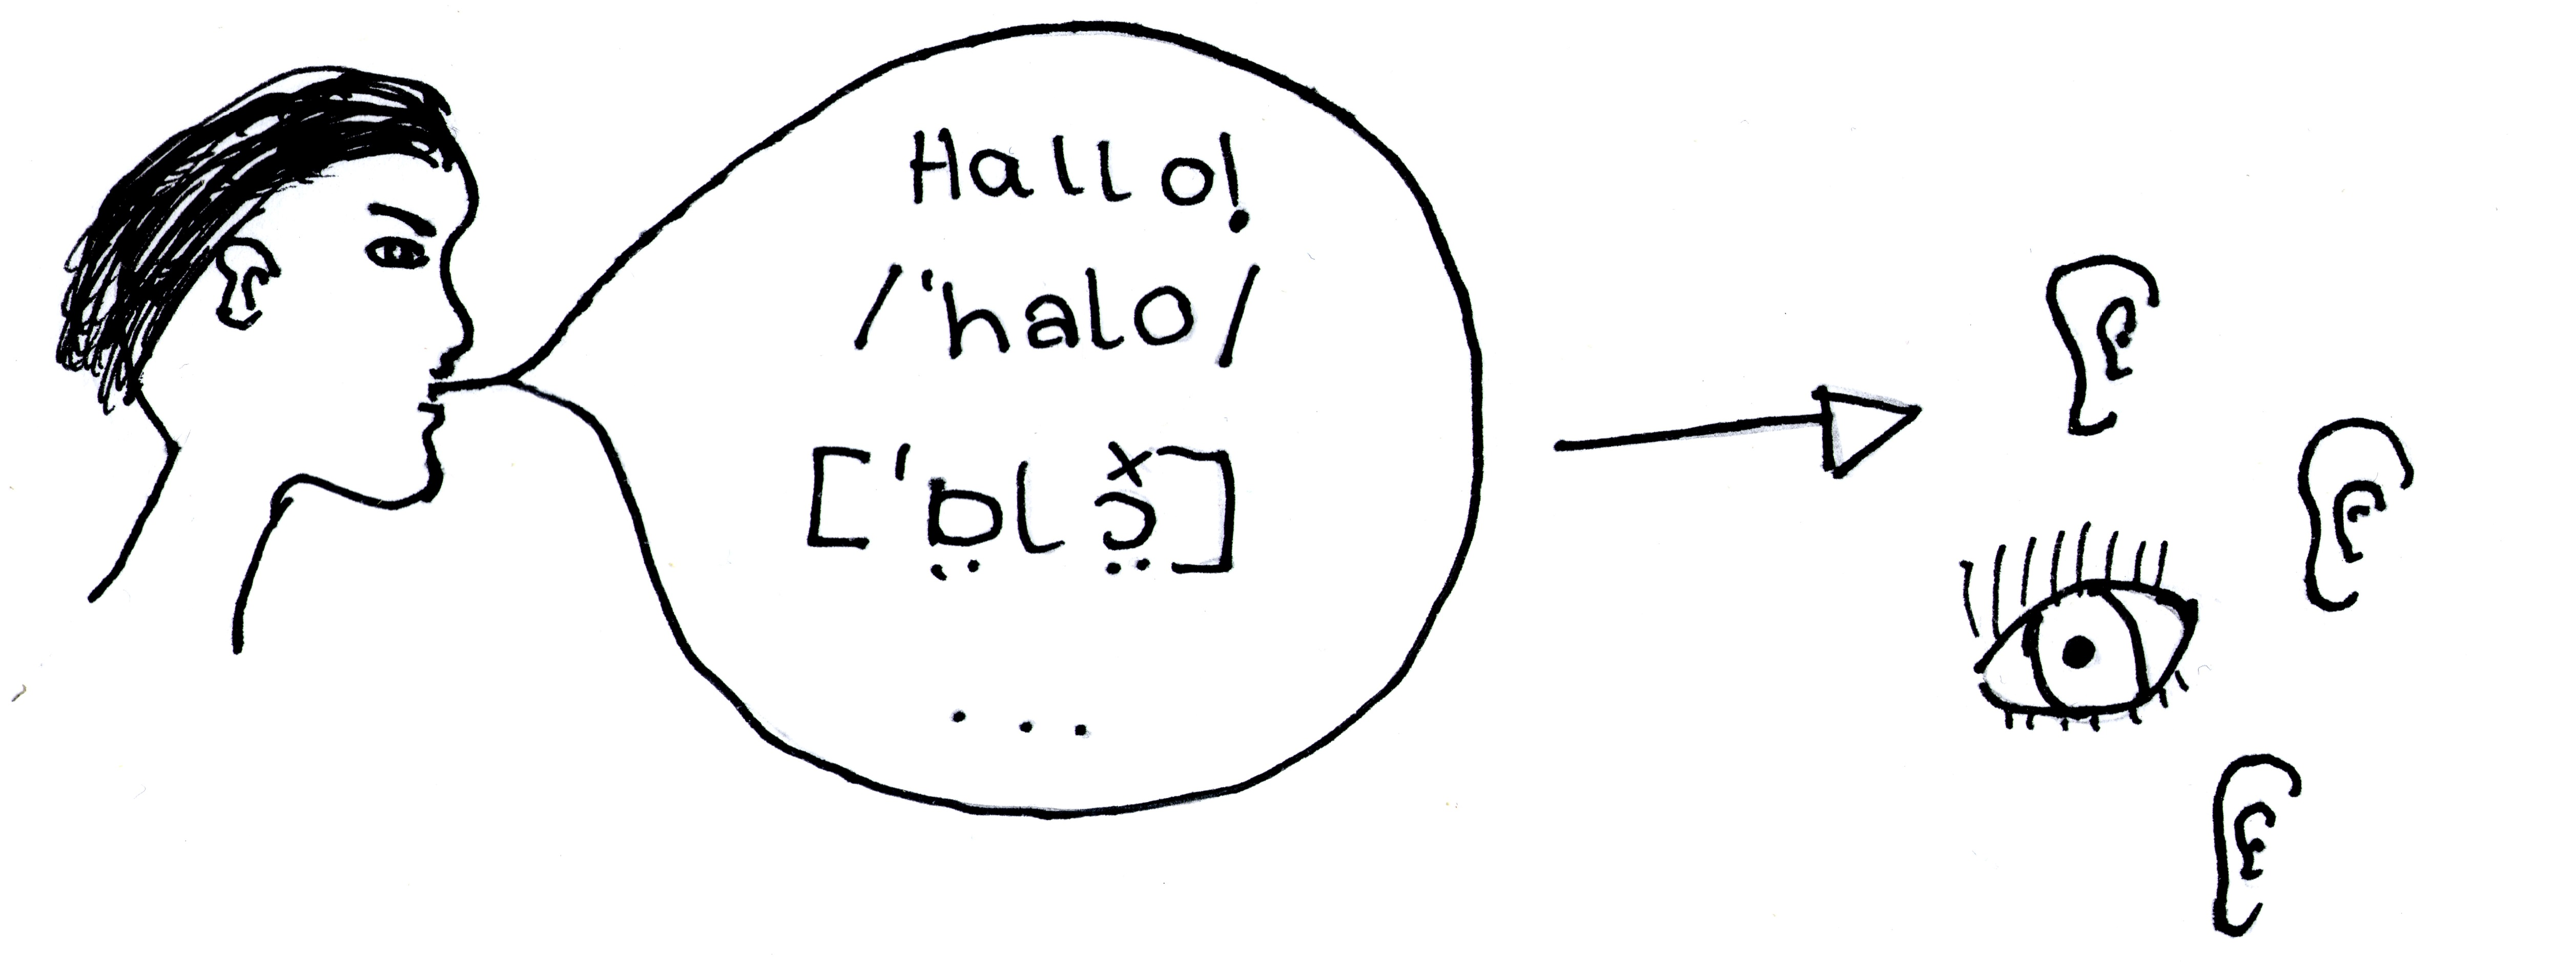
\includegraphics[width=\textwidth]{grafiken/annotationstypen/annotationstypen.jpg}
\label{t3}
\end{center}
\end{figure}
\section{Übungen}
 
1.	Öffnen Sie den ersten Satz aus ihrem Dialog in Praat ($\rightarrow$ {\tt praat.pdf}) und erzeugen Sie ein TextGrid-File mit zwei \emph{interval tiers} (1 = Wort, 2 = Segment). Öffnen Sie beide Dateien und segmentieren Sie auf der oberen Ebene (\emph{Wort-tier}) die Wörter und auf der unteren Ebene (\emph{Segment-tier}) die Sprachlaute. Für die Etikettierung der Wörter und Laute verwenden Sie bitte die Buchstaben des Deutschen. Notieren Sie ihre Beobachtung zu folgenden Fragen.\\
\newline

a.	Wie genau lassen sich Grenzen zwischen zwei Wörtern bzw. zwischen zwei Sprachlauten setzen? Notieren Sie einfache und schwierige Beispiele. \vspace{5cm}\\
b.	Wie stark hilft Ihnen ihre Sprachperzeption beim Segmentieren? \vspace{5cm}\\
\newpage
c.	Ist die Etikettierung der Sprachlaute immer eindeutig? \vspace{5cm}\\
d.	Wie gut eignen sich die Buchstaben für die Etikettierung? \vspace{5cm}\\
e.	Welche anderen akustischen Eigenschaften in der Sprachaufnahme könnte man etikettieren? \vspace*{5cm}\\
